% Adapted by M-L. Messai
\documentclass[25pt, a0paper, portrait, margin=0mm, innermargin=15mm,blockverticalspace=15mm, colspace=15mm, subcolspace=8mm]{tikzposter}

\usepackage{pgfplots}


\usepackage[utf8]{inputenc}
\renewcommand{\refname}{Références}
\usepackage{lipsum} 
\usepackage{fancyhdr}
\usepackage[scaled]{helvet}
\renewcommand\familydefault{\sfdefault} 
\usepackage[T1]{fontenc}
\usepackage{transparent} % transparence des images

\usepackage{soulutf8} % surligner du texte
%\sethlcolor{} % couleur du surlignage

\usepackage[backend=biber,
    style=numeric-comp,
    maxcitenames=1,
    maxbibnames=1,
    %backref=true
    ]{biblatex}

\usepackage{colortbl} % colorer ligne d'un tableau
\usepackage{xspace}

\usepackage{tikz}
\usetikzlibrary{arrows,shapes}

\usepackage{enumitem} % changer les points de itemize


\tikzposterlatexaffectionproofoff %enlever phrase en bas à droite
\usetheme{Simple} %différents thèmes tikzposter

% ---- Couleurs
\definecolor{mypink1}{rgb}{0.858, 0.188, 0.478}
\definecolor{titlecolor}{RGB}{74, 114, 159}
\definecolor{titledarkcolor}{RGB}{51,102,153}
\definecolor{LightGrey}{RGB}{232, 232, 232}
\definecolor{Grey}{RGB}{222, 223, 225}
\definecolor{DarkerGrey}{RGB}{215,217,219}
\definecolor{FontColor}{RGB}{131,136,138}
\definecolor{Red}{RGB}{204,0,0}
%\definecolor{L-lig}{RGB}{25,124,192}
%\definecolor{eric-lab}{RGB}{54,104,163}
\definecolor{eric-lab}{RGB}{255,73,1} 
\definecolor{eric}{RGB}{255,255,255}



\definecolor{Orange}{RGB}{240,163,10} %ERIC orange
\definecolor{Gray}{RGB}{186,200,211}
\definecolor{LightRed}{RGB}{214,98,93}
\definecolor{LightBlue}{RGB}{160,200,217}
\definecolor{LightGreen}{RGB}{130,161,119}
\definecolor{Violet}{RGB}{190,144,252}
% ----

\colorlet{blocktitlefgcolor}{eric-lab} %titre des blocks
\colorlet{blocktitlebgcolor}{Grey} %couleur des lignes blocks
%\colorlet{blockbodybgcolor}{mypink1}%????
\colorlet{blockbodyfgcolor}{FontColor} %couleur du texte dans blocks

\colorlet{innerblocktitlefgcolor}{white}
\colorlet{notefrcolor}{Red!60} % ligne autour cadre notes
\colorlet{notefgcolor}{white} % couleur police notes
\colorlet{notebgcolor}{Red!60} % BG couleur des notes


% ---- Titre
\settitle{ 
\begin{minipage}[b]{0.85\linewidth}
\vspace{2cm}
\hspace{1cm}\color{black}{ \Huge\textsc{\textbf{\@title}} \par } \vspace*{2em} \hspace{1cm}\color{black}{\LARGE \@author \par} \vspace*{2em} \hspace{1cm}\color{black}{\Large \@institute} \vspace*{2em} \end{minipage}
\hfill
\begin{minipage}{0.15\linewidth}

\vspace{-15cm}

\includegraphics[scale=0.6]{images/logos/cvlab_logo.png}
\includegraphics[scale=0.04]{images/logos/Golem_biały_logo.png}

\includegraphics[scale=0.06,trim={25cm 0 0 25cm}]{images/logos/tpx_logo.png}

\includegraphics[scale=1,trim={0 2.5cm 0 2.5cm}]{images/logos/ncbr_ideas_Mono.pdf}
 \end{minipage}}

\definetitlestyle{sampletitle}{
width=840mm, roundedcorners=0, linewidth=2pt, innersep=15pt,
titletotopverticalspace=0mm, titletoblockverticalspace=30mm
}{\begin{scope}[line width=\titlelinewidth, rounded corners=\titleroundedcorners]\draw[fill=eric-lab, color=eric]
(\titleposleft,\titleposbottom) rectangle (\titleposright,\titlepostop);
\end{scope}}



\title{\parbox{1700pt}{Towards More Realistic Membership Inference Attacks on Large Diffusion Models}}

\author{Jan Dubiński$^1$, Antoni Kowalczuk$^{1,2}$, Stanisław Pawlak$^1$, Przemysław Rokita$^1$, Tomasz Trzciński$^{1,3,4,5}$,\par \hspace{0.5cm} Paweł Morawiecki$^6$}
\institute{$^1$Warsaw University of Technology $^2$AI Society Golem $^3$Jagiellonian University $^4$IDEAS NCBR $^5$Tooploox $^6$Polish Academy of Sciences}

\usetitlestyle[]{sampletitle}
\setlength{\columnseprule}{0.4pt}
\addbibresource{Biblio/Biblio.bib}

%%%%%%%%%%%%%%%%%%%%%%%%%%%%%%%%%%%%%%%%%%%%%%%%%%%%%%%%%%%
\begin{document}
\maketitle

% --- Columns
\draw[eric-lab, line width=2mm, loosely dotted] (-13,40) -- (-13,-45); 
\draw[eric-lab, line width=2mm, loosely dotted] (15,40) -- (15,-25);

%------------------------------------------------------------------------------
% --------------------- Corpus of the poster ---------------------
\begin{columns}
\column{1}
\begin{subcolumns}
    %%%%%%%%%%%% Column 1 %%%%%%%%%%%%%
    \subcolumn{.33}
   
    % ---------------------------------MOTIVATIONS ----------
        \block{\textsc{Motivations}}{\lipsum[1]}
    

    % --------------------------------- PARTIE1----------
        \block{\textsc{Partie 1}}{\begin{itemize}
            \item item 1
            \item item 2
            \item item 3
        \end{itemize}
        
        \vspace{0.5cm}
        
        \underline{liste 2}: \begin{itemize}[label=-]
            \item item;
            \item item;
            \item item;
            \item item;
        \end{itemize} \vspace{-2cm}}
        
      % --------------------------------- PARTIE 2  ----------    
    \block{\textsc{Partie 2}}{
        
        \tikzstyle{na}=[baseline=-.25ex]
        \tikzstyle{every picture}+=[remember picture]
        \vspace{0.5cm}
        
        \innerblock{Avec titre}{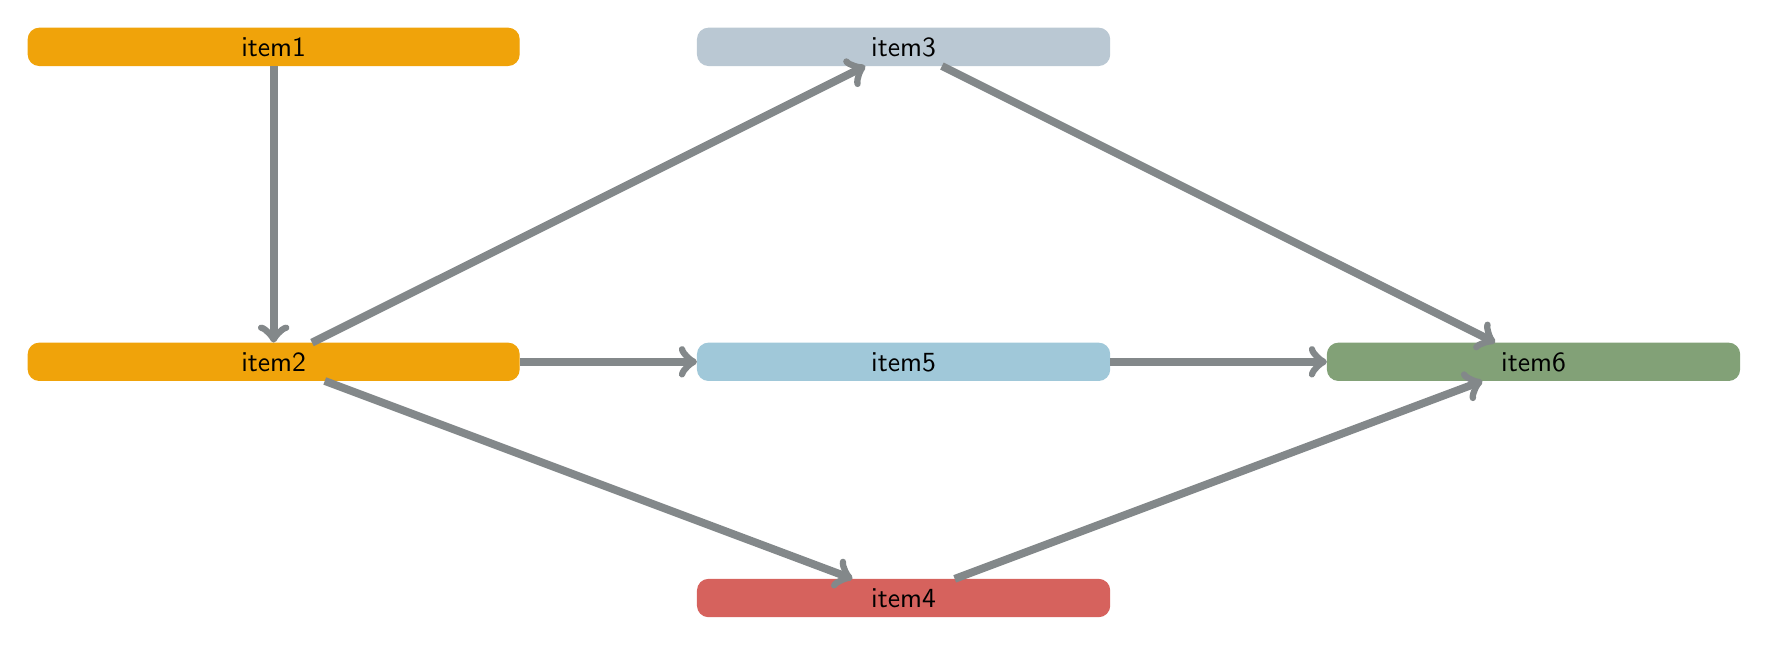
\begin{tikzpicture}
    \node[draw=Orange,fill=Orange,text=black,text width=6cm, rounded corners, text centered] (item1) at (2,4) {item1};
    
    \node[draw=Orange,fill=Orange,text=black,text width=6cm,rounded corners, text centered] (item2) at (2,0) {item2};
    
    \node[draw=Gray,text width=5cm,fill=Gray,rounded corners, text centered, text=black] (item3) at (10,4) {item3};
    
    \node[draw=LightRed,text width=5cm,fill=LightRed,text=black,rounded corners, text centered] (item4) at (10,-3) {item4};
    
    \node[draw=LightBlue,text width=5cm,text=black,fill=LightBlue,rounded corners, text centered] (item5) at (10,0) {item5};
    
    \node[draw=LightGreen,fill=LightGreen,text=black,text width=5cm,rounded corners, text centered] (item6) at (18,0) {item6};
    
    \draw[->, line width=1mm, draw=FontColor] (item1) to (item2);
    \draw[->,line width=1mm, draw=FontColor] (item2) to (item3);
    \draw[->,line width=1mm,draw=FontColor] (item2) to (item4);
    \draw[->,line width=1mm,draw=FontColor] (item2) to (item5);
    \draw[->,line width=1mm,draw=FontColor] (item3) to (item6);
    \draw[->,line width=1mm,draw=FontColor] (item5) to (item6);
    \draw[->,line width=1mm,draw=FontColor] (item4) to (item6);
    
    \end{tikzpicture}
    
    
        } 
        \vspace{0.5cm}
        \lipsum[1]
            
          \vspace{-2cm}}
          
    %%%%%%%%%%%%%%% Column 2 %%%%%%%%%%%%%
    \subcolumn{.33}
    
        % ---------------------------------  PARTIE 3----------
        \block{\textsc{Partie 3}}{\innerblock{}{
        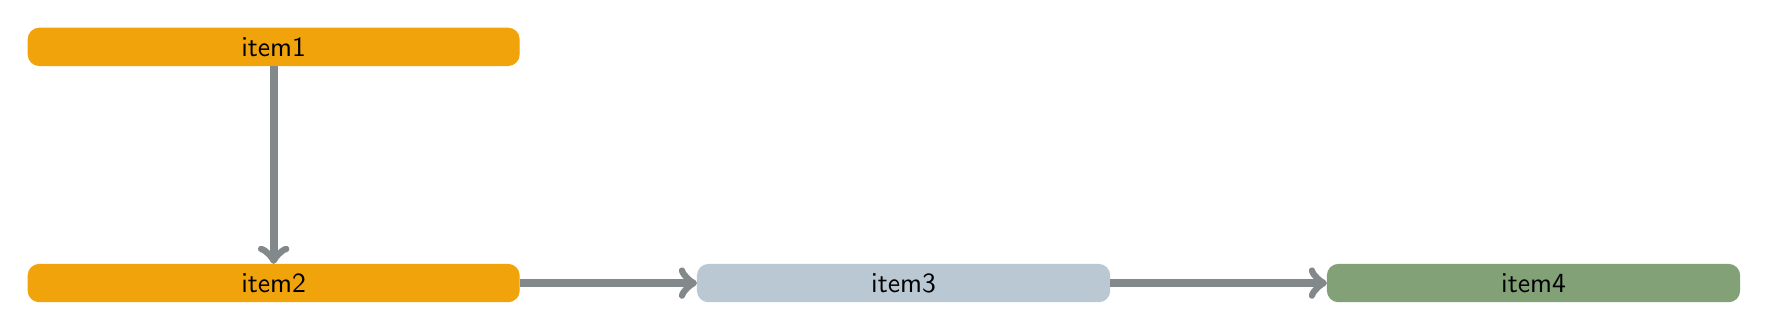
\begin{tikzpicture}
    \node[draw=Orange,fill=Orange,text=black,text width=6cm, rounded corners, text centered] (item1) at (2,4) {item1};
    
    \node[draw=Orange,fill=Orange,text=black,text width=6cm,rounded corners, text centered] (item2) at (2,1) {item2};
    
    \node[draw=Gray,text width=5cm,fill=Gray,rounded corners, text centered, text=FontColor, text=black] (item3) at (10,1) {item3};
    
    \node[draw=LightGreen,text width=5cm,fill=LightGreen,text=black,rounded corners, text centered] (item4) at (18,1) {item4};
    
    \draw[->, line width=1mm, draw=FontColor] (item1) to (item2);
    \draw[->,line width=1mm, draw=FontColor] (item2) to (item3);
    \draw[->,line width=1mm, draw=FontColor] (item3) to (item4);
    
    \end{tikzpicture}} \vspace{2cm} \lipsum[2]
        \vspace{-2cm}}
            
        \note[targetoffsetx = 3cm, targetoffsety = 1cm, angle = 20, connection]{\textbf{exemple de note}}

        
    % --------------------------------- PARTIE 4  ----------
        \block{\textsc{Partie 4}}{ %\lipsum[3]
        %\vspace{-2cm}
        
        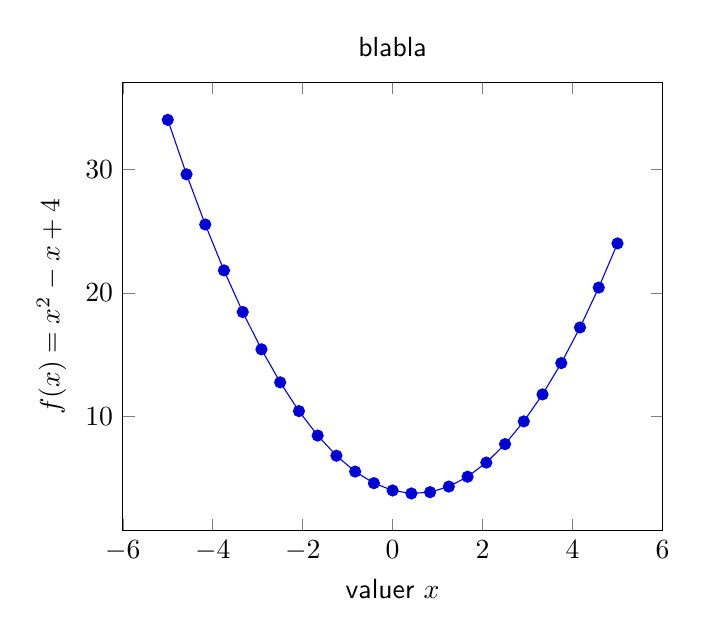
\begin{tikzpicture}
        \begin{axis}[ 
        title={blabla},
        xlabel={valuer $x$},
        ylabel={$f(x) = x^2 - x +4$}
        ] 
        \addplot {x^2 - x +4}; 
        \end{axis}
        \end{tikzpicture}
       %\vspace{2cm}
        \begin{tikzpicture}
        \begin{axis}
        \addplot[color=red]{exp(x)};
        \end{axis}
        \end{tikzpicture}
        
        }
    
  
 % ------------------------------------ PARTIE 5------------
        \block{\textsc{Partie 5}}{\lipsum[1]  
        
        \hspace{-6cm}
\parbox{1700pt}{\begin{tikzfigure}[]
         \renewcommand{\arraystretch}{1.3}
        \begin{tabular}{|p{11.5cm}|p{11cm}|p{20cm}|r|}
        \hline
        \rowcolor{eric}\textcolor{black}{\textbf{Titre} } & \textcolor{black}{\textbf{Titre}} & \textcolor{black}{\textbf{Titre}} & \textcolor{black}{\textbf{Durée}}    \\ \hline
        
        \rowcolor{LightGrey} Ligne 1 & Case 1 & & 2\,h \\ \hline 
        
        \rowcolor{white}Ligne 2 & Case 2 & & 450\,h  \\ \hline
        
        \rowcolor{LightGrey} Ligne 1 & Case 1 & & 2\,h \\ \hline 
        
        \rowcolor{white}Ligne 2 & Case 2 & & 450\,h \\ \hline
        
        \rowcolor{LightGrey} Ligne 1 & Case 1 & &2\,h \\ \hline 
        
        \rowcolor{white}Ligne 2 & Case 2 & &450\,h \\ \hline
        
        \rowcolor{LightGrey}\textbf{Total} &  & &\textbf{1000\,h\,58} \\ \hline 
        \end{tabular}
        
        %\vspace{0.6cm} * Commentaire 
        
        \end{tikzfigure}} 
            \vspace{-2cm}}

 
 %%%%%%%%%%%%%%%%%%%%%%%% Column 3 %%%%%%%%%%%%%%%%%%%%%%%%%   
    \subcolumn{.33}

    % ---------------------------------------------
        \block{\textsc{Conclusion}}{
        \lipsum[1]
        
        \vspace{0.5cm}
        \lipsum[2] \cite{ref1}
        \vspace{0.5cm}}

    % ----------------------------------------------
        \block{}{
        \vspace{3cm}
            \textbf{SPA}: Société Protectrice des Animaux $\bullet$
            \textbf{CAF}: Caisse d'Allocations Familiales $\bullet$
            \textbf{WER}: Word Error Rate }   
    
    \end{subcolumns}
    

    % ---------------------------------  References ----------
    \block{}{\vspace{1cm}
       \printbibliography}
       \end{columns}

% ----------------- Footer -------------
\node [above right, text=white,outer sep=45pt,minimum width=\paperwidth, align=center, draw, fill=titledarkcolor, color=Orange] at (-43.6,-61) { \textcolor{white}{\normalsize Contact: prenom.nom@univ-lyon2.fr}};

\end{document}
